\documentclass[12pt, a4paper]{article}

% language
\usepackage[american]{babel}
\usepackage[utf8]{inputenc}

% bib
\bibliographystyle{plainurl}

\usepackage{amsmath}
\usepackage{amsfonts}
\usepackage{url}

% I need them :-)
\usepackage[plainpages=false]{hyperref}
\hypersetup {
   pdfauthor={Johannes Wei\ss},
   pdftitle={Dimplomarbeit -- Roadmap},
   pdfsubject={Diploma Thesis Roadmap},
   pdfkeywords={KIT, crypto, diploma thesis, roadmap}
}
\usepackage{listings}
\usepackage{color}
\usepackage{tikz}

%
% SPECIAL IMPORTS
%
\usepackage{xparse}
\usepackage{boxedminipage}


%
% GENERAL
%

% environments
\NewDocumentEnvironment{JWboxed}{mm}%
  {\begin{figure}[ht]%
   \small%
   \begin{boxedminipage}{\linewidth}%
  }%
  {\end{boxedminipage}%
   \caption{#1}%
   \label{#2}%
   \end{figure}%
  }

% functionality
\newenvironment{JWfunc}[3]%
{\begin{JWboxed}{#2}{#3}%
 \begin{center}\textbf{{Functionality #1}}\end{center}%
}%
{\end{JWboxed}}

\newenvironment{JWfuncSteps}[0]%
{\begin{itemize}}{\end{itemize}}

\newcommand{\JWfuncSym}[2]{$\mathcal{F}^\mathrm{#1}_\mathrm{#2}$}

%protocol
\newenvironment{JWprotocol}[3]%
{\begin{JWboxed}{#2}{#3}%
 \begin{center}\textbf{{Protocol #1}}\end{center}%
}%
{\end{JWboxed}}

\newenvironment{JWprotoSteps}[0]%
{\begin{enumerate}}{\end{enumerate}}

\newcommand{\JWprotoPhase}[1]{\paragraph{#1}}

\newcommand{\JWprotoSym}[2]{$\Pi^\mathrm{#1}_\mathrm{#2}$}

%misc
\newcommand{\JWtodo}[1]{\fbox{TODO: #1}}
\newcommand{\JWmsgTwo}[2]{(\texttt{#1}, \texttt{#2})}

%chapters
\newcommand{\JWlone}[1]{\chapter{#1}}
\newcommand{\JWltwo}[1]{\section{#1}}
\newcommand{\JWlthree}[1]{\subsection{#1}}
\newcommand{\JWlfour}[1]{\subsubsection{#1}}
\newcommand{\JWlfive}[1]{\paragraph{#1}}
\newcommand{\JWlsix}[1]{\subparagraph{#1}}


%
% SPECIALIZED SHORTCUTS
%
\newcommand{\JWprotoSymOPE}[0]{\JWprotoSym{}{OPE}}
\newcommand{\JWfuncSymOPE}[0]{\JWfuncSym{(q, k)}{OPE}}
\newcommand{\JWfieldGeneral}[0]{\mathbb{F}_q^k}
\newcommand{\JWpOne}[0]{Goliath}
\newcommand{\JWpTwo}[0]{David}


\title{Diplomarbeit -- Roadmap}

\author{Johannes Weiß}

\begin{document}

\maketitle

This writing describes the process of securely evaluating arithmetic functions
such as $f(x_G,x_D) = ...$ over finite fields. The main building block is the
David \& Goliath OAFE protocol\cite{davidgoliath}.

\section{Using Affine Randomized Encodings}
\label{sec:are}

As the main building block OAFEs---as provided by the David \& Goliath protocol
\cite{davidgoliath}---are used. However, the first step is to securely express
the input function $f(x_G, x_D)$ in terms of affine functions. These affine
functions can then be securely evaluated using OAFEs. At a first glance, the
task of expressing a general function $f(x_G, x_D)$ using affine functions may
seem a rather easy task. The challenge is to do it securely: The other party
should obviously not be able to learn $G$ when it is given the linear functions
expressing the partly evaluated function $f(G, x_D)$ (value $G$ already set).
Additionally, the process should work non--interactively: The first party fixes
its input $x_G = G$, partly evaluates $f(G, x_D)$, transforms it to affine
functions and sends them as OAFEs to the second party. The affine functions
themselves are either a constant or hidden inside an OAFE calculation. After the
second party provided their input $x_D$ to the OAFEs, it gets (from the OAFEs)
the evaluated results of the linear functions. The second party is now---using a
provided decoder---able to securely and fully evaluate $f(x_G, x_D)$ using only
the values received from the OAFEs and the constants. Neither party will learn
more of the other party's input than the final result will tell it anyway.

The transformation from general functions to affine functions used in this
thesis will lead to a slightly modified form of \emph{Decomposable Affine
Randomized Encodings} (DAREs) \cite{gac2012} only called \emph{Affine Randomized
Encoding} (ARE) in this thesis. The modification is necessary because this
thesis uses OAFEs to evaluate the DAREs and does therefore not depend on the
learning with errors (LWE) problem. This leads to further changes: The
\emph{affinization gadget} \cite{gac2012} is modified and the
\emph{key--shrinking gadget} \cite{gac2012} is not needed.

\noindent{}The following sections will describe the whole process.


\subsection{Affine Randomized Encodings}
\label{sec:affinization-gadget}

\subsubsection{Definitions}
\label{sec:affinization_definitions}

An \emph{Linear Randomized Expression} (LRE) is an element of the set
$\mathcal{F}_{AR}$ ($K$ a finite field), an \emph{Affine Randomized Encoding}
(ARE) an element of the set $\mathcal{E}_{AR}$. One important constraint has to
hold for all LREs and therefore for all AREs, too: After fully evaluating a LRE,
i.e. replacing the variable by its actual value, the now constant LRE should
reveal no more information that the result of a full decoding of the respective
ARE. The safety is proven in \emph{How to Garble Arithmetic Circuits}
\cite{gac2012}.

\begin{align*}
  \mathcal{V} = & \{ x \mid x~\text{a variable over}~K \} \\
%
  \mathcal{F}_{AR} = & \{ s \cdot x + i \mid s, i \in K, x \in \mathcal{V} \}
  \cup \{ v \mid v \in K \} \\
%
  \mathcal{E}_{AR} = & \{ (M, A) \mid
    M \subseteq \mathcal{F}_{AR} \times \mathcal{F}_{AR},
    A \subseteq, \mathcal{F}_{AR};
    A, M~\text{finite multi--sets} \}
%
\end{align*}


\subsubsection{Encoding}
\label{sec:affinization_encoding}

\begin{itemize}

\item A function $f_1(x_1, x_2) = x_1 + x_2$ can be securely encoded by
$ENC_A(f_1, r)$; $r \in K$ being uniformly at random

\item A function $f_2(x_1, x_2, x_3) = x_1 \cdot x_2 + x_3$ can be securely
encoded by $ENC_M(f_2, r_1, r_2, r_3, r_4)$; $r_1, r_2, r_3, r_4 \in K$ being
uniformly at random
\end{itemize}

\begin{align*}
ENC_A(f_1, r) = \Big( & \emptyset, (x_1 + r, 1 \cdot x_2 - r)\Big) \\
ENC_M(f_2,  r_1, r_2, r_3, r_4) = \Bigg( & \bigg\{
\begin{pmatrix}1 \cdot x_1 - r_1\\1 \cdot x_2 - r_2\end{pmatrix} \bigg\}\\
,& \bigg\{r_2 \cdot x_1 -r_1r_2+r_3 \\
&\ ,\ r_1 \cdot x_2 + r_4 \\
&\ ,\ 1 \cdot x_3-r_3-r_4\bigg\} \Bigg)
\end{align*}


\subsubsection{Decoding}
\label{sec:affinization_decoding}

Decoding a fully evaluated ARE $\mathcal{E}_{AR} = \{(M,A)\}$ as $r =
DEC(\mathcal{E}_{AR})$ is
straightforward:

\begin{align*}
M' &= \Bigg\{ m_1 \cdot m_2\ \Bigg|\ \begin{pmatrix}m_1\\m_2\end{pmatrix}
\in M \Bigg\} \\
r & = \sum_{a \in A} a + \sum_{m \in M'} m
\end{align*}


\subsection{Randomized Variables}
\label{sec:rv}

Whenever a circuit is not directly transformable to one single ARE, sub--AREs
get replaced by \emph{Randomized Variables} (RV). RVs are just (sub--)ARE that
get transmitted to the second party (see section \ref{sec:are}) which
fully evaluates them and saves the result just like an ordinary input variable
(such as $x_D$). Following AREs may then use the RVs as pseudo--inputs. But
since a ARE reveals as much information as its decoded form, the original ARE
cannot just be transmitted as the final overall ARE. That would reveal
intermediate information. Therefore, RVs get an additional garbling step: Say
the following property would hold for a variable $v$ being the decoded value of
an ARE $e$:

\begin{align*}
  v = DEC(e \in \mathcal{E}_{AR})
\end{align*}

\noindent{}Then a modified ARE $\hat{e} \in \mathcal{E}_{AR}^+$ decoding to a
value $\hat{v}$

\begin{align*}
\hat{v} = \alpha \cdot (v + \beta) = DEC(\hat{e})
\end{align*}

\noindent{}with secret keys---known only by the first party---$\alpha$ and
$\beta$ would get transmitted.


\subsection{Checked Bi--Randomized Variables}
\label{sec:cbrv}

The RV technique (see section \ref{sec:rv}) prevents the
second party from directly gaining intermediate information. But, for a
corrupted second party, there is still the possibility of gaining supplemental
information: The second party could forge an RV value before applying it to one
of the following AREs. This will not directly reveal additional information
because the second party does not know the encryption keys used for the RV. So,
the second party is unaware of the decoded value of the RV. But except for a
negligible probability $\left(\frac{1}{Char(K)}\right)$, the decoded value is
non--zero.  The knowledge of a random but non--zero value can then be used to
test a secret input of the first party against zero. \JWtodo{Beispiel hierfür,
siehe z.B. Google Doc.}

To address this issue, a similar but secure technique is proposed in here: The
\emph{Checked Bi--Randomized Variables} (CBRVs). Every input made to an OAFE by
the second party is encoded as a CBRV. The CBRVs $\hat{v}$ corresponding to a
value $v$ are: ($\alpha_l, \alpha_r \in K \setminus \{0\}; \beta, \beta' \in K$)

\begin{align*}
  \widetilde{v} = (\widetilde{v_1}, \widetilde{v_2}) =
  (\alpha_l \cdot v + \beta, \alpha_r \cdot v + \beta')
\end{align*}

\noindent{} $\alpha_l$ and $\alpha_r$ are the \emph{static keys}, $\beta$ and
$\beta'$ the \emph{dynamic keys} of the CBRV. The static keys are (non--zero)
numbers uniformly at random but constant for the entire procedure. $\beta$ and
$\beta'$ are fresh, independent and uniformly distributed random numbers for
every CBRV component generated while processing a circuit. Only the first party
knows these secret keys. The initial CBRVs used to feed the second party's
regular inputs party are generated using an OAFE that evaluates for every input
$x$:

\begin{align*}
  \widetilde{x} = (\alpha_l \cdot x + \beta_1, \alpha_r \cdot x + \beta_2)
\end{align*}

The first party is---because it generates and knows all the keys---in possession
of the encoding and decoding functions

\begin{align*}
  E(x) &= \left(\alpha_l \cdot x + \beta_1, \alpha_r \cdot x + \beta_2\right) \\
  D(\widetilde{x}) &= \left(\frac{\widetilde{x_1} - \beta_1}{\alpha_l},
                       \frac{\widetilde{x_2} - \beta_2}{\alpha_r}\right)
\end{align*}

A CBRF $\widetilde{x}$ is well--formed iff the tuple $D(\widetilde{x})$ consists
of two equal values.


\subsection{Checked Bi-Randomized Affine Encodings}
\label{sec:cbrae}

\emph{Checked Bi-Randomized Affine Encodings} (CBRAEs) are very similar to AREs
(section \ref{sec:are}) but use CBRVs (section \ref{sec:cbrv}) instead of plain
values and RVs (section \ref{sec:rv}).

\begin{align}
  \mathcal{V} = & \{ x \mid x~\text{a variable over}~K \} \\
%
  \mathcal{F}_{AR} = & \{ s \cdot x + i \mid s, i \in K, x \in \mathcal{V} \}
  \cup \{ v \mid v \in K \} \\
%
  \mathcal{B}_{AR} = & \{ (\alpha_l \cdot f + \beta, \alpha_r \cdot f + \beta' )
  \mid \alpha_l, \alpha_r \in K \setminus \{0\}; \beta, \beta' \in K; f \in
  \mathcal{F}_{AR} \} \\
%
  \label{rel:cbrae}
  \mathcal{E}_{AR} = & \{ (M, A) \mid
    M \subseteq \mathcal{B}_{AR} \times \mathcal{B}_{AR},
    A \subseteq, \mathcal{B}_{AR};
    A, M~\text{finite multi--sets} \}
%
\end{align}

\noindent Intuitively, $\mathcal{V}$ are ordinary inputs and CBRVs,
$\mathcal{F}_{AR}$ represent linear, encrypted particles that encode parts of
the final function. To prevent illegal information gaining by a corrupted second
party, $\mathcal{B}_{AR}$ represents checked and encoded intermediate values
(see section \ref{sec:cbrv}) that can safely be passed to untrusted parties.
$\mathcal{E}_{AR}$ is the final encoding, powerful enough to encode arbitrary
arithmetic functions. $\mathcal{E}_{AR}$s are full--blown CBRAEs as presented in
this thesis. The decoding part remains as in section
\ref{sec:affinization_decoding}. The result will be a tuple that can then be
decoded in one last step as in section \ref{sec:eval-final-value}.


\subsubsection{Encoding Arithmetic Operations as CBRAEs}
\label{sec:encode-cbrae}

As in section \ref{sec:cbrv} we assume the universal decoding function
$D(\widetilde{x})$. With CBRVs, the arithmetic operations are mapped as follows:


\paragraph{Addition}

Two CBRVs $\widetilde{x}$ and $\widetilde{y}$ can be added componentwise to
$\widetilde{z} = \left(\widetilde{x_1} + \widetilde{y_1}, \widetilde{x_2} +
\widetilde{y_2}\right)$. Since the first party is in
possession of the encryption keys ($\widetilde{x} = \left(\alpha_l \cdot x +
\beta_1, \alpha_r \cdot x + \beta_2\right)$, $\widetilde{y} = \left(\alpha_l
\cdot x + \beta_3, \alpha_r \cdot x + \beta_4\right)$) it's obvious that:
$\widetilde{z} = \left(\alpha_l \cdot (x+y) + (\beta_1 + \beta_3), \alpha_r
\cdot (x+y) + (\beta_2 + \beta_4)\right)$ and $\widetilde{z}$ is well--formed.

Having two CBRAEs, they can be added by simply concatenating the multiplicative
($M$ in relation \ref{rel:cbrae}) and additive ($A$) parts.


\paragraph{Addition -- Alternative Form}

The alternative addition form is
$\widetilde{z} =
\left( E\left(D(\widetilde{x_1}) + D(\widetilde{y_1})\right),
       E\left(D(\widetilde{x_2}) + D(\widetilde{y_2})\right)
\right)$.
Since $E(x)$ and $D(x)$ are both linear functions,
$E\left(D(\ldots) +D(\ldots)\right)$
are linear expressions, too that can be evaluated using two OAFE calls.


\paragraph{Multiplication}

As for ordinary AREs, the multiplication is not as powerful as the addition,
direct multiplication of two CBRAEs is not possible. CBRAE multiplication is
done using CBRVs sent to the second party. Then, these CBRVs get multiplied as
described here:

\begin{align*}
  e & \in \mathcal{E}_{AR}; \widetilde{x}, \widetilde{y} \in \mathcal{B}_{RV};
  r_1, r_2, r_3, r_4, r_5, r_6, r_7, r_8 \in K;
  \alpha_l, \alpha_r \in K \setminus \{0\} \\
  %
  e & = \widetilde{x} \otimes \widetilde{y} \\
  %
  e & = \Bigg(\Big\{\big( \alpha_l \cdot D(\widetilde{x_1}) - r_1,
                          \alpha_r \cdot D(\widetilde{x_2}) -r_5 \big) \\
    &\qquad ,     \big(   1        \cdot D(\widetilde{y_1}) - r_2,
                          1        \cdot D(\widetilde{y_2}) - r_6 \big) \Big\}\\
    &\qquad   \Big\{\big( \alpha_lr_2 \cdot D(\widetilde{x_2}) + r_3,
                          \alpha_rr_2 \cdot D(\widetilde{x_1}) + r_7 \big) \\
    &\qquad ,       \big ( r_1        \cdot D(\widetilde{y_2}) + r_4,
                           r_5        \cdot D(\widetilde{y_1}) + r_8 \big)
              \Big\}\Bigg) \\
\end{align*}

The decryption keys of $e$ are $\alpha_l$, $\alpha_r$ (static keys) and
$\beta = r_1r_2 + r_3 + r_4$, $\beta' = r_5r_6 + r_7 + r_8$ (dynamic keys).


\subsubsection{Evaluating the Final Value}
\label{sec:eval-final-value}

In contrast to the RV technique (section \ref{sec:rv}), the
CBRV technique encodes all values. So even the final value, the result of the
entire calculation, is encrypted. The encryption works as follows: After
evaluation the last CBRAE, the second party is in possession of an CBRV tuple
$\widetilde{r} = (\widetilde{r_1}, \widetilde{r_2})$. The second party then
calculates $\widehat{r} = \widetilde{r_1} + \widetilde{r_2}$ and decodes it to
$r$ using a specific final OAFE. This OAFE was set up by the first party at the
beginning as follows: Assuming $\widetilde{r_1}$ was encrypted using $(\alpha_l,
\beta_{r_1})$ and $\widetilde{r_2}$ was encrypted using $(\alpha_r,
\beta_{r_2})$ the first party knows $\widehat{r}$ has to be encrypted using
$(\alpha_l + \alpha_r, \beta_{r_1} + \beta_{r_2})$. Given this knowledge the
final OAFE setup is $\frac{1}{\alpha_l + \alpha_r} \cdot \widehat{r} -
\frac{\beta_{r_1} + \beta_{r_2}}{\alpha_l + \alpha_r}$.

The gain of this technique is that the second party is getting caught if it
cheated. If it cheated somewhere in the process and forged one of its CBRV
tuples $\widetilde{x} = (\widetilde{x_1}, \widetilde{x_2})$ to $\widetilde{x'} =
(\widetilde{x_1} + \Delta_1, \widetilde{x_2} + \Delta_2)$, the CBRV
$\widetilde{x'}$ becomes---except for a negligible probability---non--wellformed
(see section \ref{sec:cbrv}). The result is that the final
result will become uniform randomness (assuming $\widetilde{x}$ is forged to
$\widetilde{x'_1} = \widetilde{x_1} + \Delta_1$ and $\widetilde{x'_2} =
\widetilde{x_2} + \Delta_2$):

\begin{align*}
  \widehat{x'} = & \widetilde{x'_1} + \widetilde{x'_2} = \widetilde{x_1} +
  \Delta_1 + \widetilde{x_2} + \Delta_2 \\
  %
  \Rightarrow x' = & \frac{1}{\alpha_l + \alpha_r} \cdot \widehat{x'} -
  \frac{\beta_{x_1} +
  \beta_{x_2}}{\alpha_l + \alpha_r} \\
  %
  \Leftrightarrow x' = & \frac{\widetilde{x_1} + \Delta_1 +
  \widetilde{x_2} + \Delta_2}{\alpha_l + \alpha_r} -
  \frac{\beta_{x_1} +\beta_{x_2}}{\alpha_l + \alpha_r}\\
  %
  \Leftrightarrow x' = & \frac{(\alpha_l x + \beta_{x_1}) + \Delta_1 +
  (\alpha_r x + \beta_{x_2}) + \Delta_2}{\alpha_r + \alpha_l} -
  \frac{\beta_{x_1} +\beta_{x_2}}{\alpha_l + \alpha_r} \\
  %
  \Leftrightarrow x' = & \frac{(\alpha_l+\alpha_r)x + (\beta_{x_1}+\beta_{x_2} +
  \Delta_1+\Delta_2)}{\alpha_l+\alpha_r} -
  \frac{\beta_{x_1} +\beta_{x_2}}{\alpha_l + \alpha_r} \\
  %
  \Leftrightarrow x' = & x + \frac{\beta_{x_1}+\beta_{x_2}}{\alpha_l+\alpha_r}
  + \frac{\Delta_1 + \Delta_2}{\alpha_l + \alpha_r} -
  \frac{\beta_{x_1}+\beta_{x_2}}{\alpha_l + \alpha_r} \\
  %
  \Leftrightarrow x' = & x + \frac{\Delta_1 + \Delta_2}{\alpha_l + \alpha_r}
\end{align*}


%
% PREPARING CBRAE EVALUATION USING OAFEs
%
\subsection{Preparing CBRAE Evaluation Using OAFEs}
\label{sec:prep-eval}

After transforming an arithmetic expressing to CBRAEs (section \ref{sec:cbrae})
assigned to CBRVs (section \ref{sec:cbrv}) the OAFEs (\cite{davidgoliath}) need
to be set up. First of all, two separate OAFEs have to be set up for each CBRV
that can be evaluated later on as soon the value is known. The OAFEs are
configured with the linear expressions inside the CBRAEs. Each CBRAE is then
transformed to two \emph{Encoding Descriptors} (EDs) that have the same
structure as the CBRAEs but contain OAFE references instead of linear
expressions. Therefore, each CBRAE assigned to a CBRV gets transformed to two
EDs, because of the tuple form of the CBRVs and CBRAEs.


%
% OBLIVIOUS POLYNOMIAL EVALUATION
%
\subsection{Oblivious Polynomial Evaluation}
\label{sec:ope}

This section describes the whole process of obliviously evaluating a univariate
polynomial $f(x) = \sum_{i=1}^k a_ix^i$. The first party (\JWpOne{}) fixes the
polynomial and configures the OAFEs, the second party (\JWpTwo{}) chooses input
$x$. Eventually, \JWpTwo{} will learn $f(x)$ but not the polynomial's
coefficients $a_i$. \JWpOne{} will not learn anything at all.

The first step is to transform $f$ to OAFEs and EDs (section
\ref{sec:prep-eval}). The OAFEs are then sent to the second party (\JWpTwo{})
using the David \& Goliath protocol \cite{davidgoliath}, the EDs are sent to the
second party using an encrypted channel aswell.

After having received the OAFEs and EDs, the first party (\JWpOne{}) is not
needed anymore and the second party (\JWpTwo{}) can evaluate the polynomial by
itself. To run the evaluation, the second party just evaluated the EDs one by
one. After each evaluation, it queries the respective OAFE (should be the next)
with the value if did just calculate. After having calculated the last to ED
values, it queries a special OAFE (see section \ref{sec:eval-final-value}) using
the addition of the values of the last two EDs. The evaluation of the special
OAFE is the result of the whole computation.
%
% PROTOCOL DESCRIPTION
%
\subsection{Protocol Description} \label{sec:protocol-description}

\begin{JWfunc}%
  {\JWfuncSymOPE}%
  {The ideal $\JWfieldGeneral{}$-OPE functionality \JWfuncSymOPE{}}%
  {fig:func-ope}

  Parametrized by a finite field size $q$ and maximal polynomial degree $k$.

  \begin{JWfuncSteps}

  \item Upon receiving input $a \in \mathbb{F}_q^k$ from \JWpOne{}, verify that
    there is no stored input from \JWpOne{}, yet; else ignore that input. Next
    record $a$ and send \JWmsgTwo{processing}{\JWpOne{}} to the adversary.

  \item Upon receiving input $x \in \mathbb{F}_q$ from \JWpTwo{}, verify that
    there is no stored input from \JWpTwo{}, yet; else ignore that input. Next
    record $x$ and send \JWmsgTwo{processing}{\JWpTwo{}} to the adversary.

  \item Upon receiving a message \JWmsgTwo{delivery}{\JWpTwo{}} from the
    adversary, verify that \JWpTwo{} and \JWpOne{} have both already provided
    some input; else ignore that message. Next, compute $y \leftarrow
    \sum_{i=1}^k a_ix^i$ and send $y$ to \JWpTwo{}.

  \end{JWfuncSteps}
\end{JWfunc}

\begin{JWboxed}%
  {Graphical Representation of \JWfuncSymOPE}%
  {fig:graph-ope}

  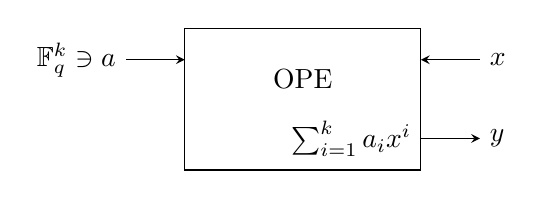
\begin{tikzpicture}[>=stealth]

    \node (OPE) at (8.5,0) {OPE};
    \draw (OPE) +(-1.5,-1.15) rectangle +(1.5,0.65);

    \draw [<-] (OPE) ++(-1.5,0.25) node [anchor=west] {} -- +(-0.75,0) node
    [anchor=east] {$\JWfieldGeneral \ni a$};

    \draw [<-] (OPE) ++(1.5,0.25) node [anchor=east] {} -- +(0.75,0) node
    [anchor=west] {$x$};

    \draw [->] (OPE) ++(1.5,-0.75) node [anchor=east] {$\sum_{i=1}^k a_ix^i$}
    -- +(0.75,0)
    node [anchor=west] {$y$};

  \end{tikzpicture}
\end{JWboxed}

\begin{JWprotocol}%
  {\JWprotoSymOPE}%
  {Protocol: Oblivious Polynomial Evaluation}%
  {fig:proto-ope}

  \JWprotoPhase{Setup:}

  \begin{JWprotoSteps}

  \item \JWpOne{} generates OAFEs and EDs (see section \ref{sec:prep-eval})

  \item \JWpOne{} sends the OAFEs and EDs to \JWpTwo{}

  \end{JWprotoSteps}


  \JWprotoPhase{Evaluation:}

  \begin{JWprotoSteps}

  \item Upon receiving the OAFEs and EDs, \JWpTwo{} evaluates the EDs one by one
    and saved the values needed for further computations

  \item After the Evaluation, \JWpTwo{} adds the values of the last two EDs and
    queries a special last OAFE with that value. The then received new value is
    the result of the computation $y = \sum_{i=1}^k a_ix^i$.

  \end{JWprotoSteps}

\end{JWprotocol}


\section{Using Linear Bijection Straight--Line Programs}
\label{sec:using-lbs}

The first approach taken in this thesis to transform general formulas to affine
functions suitable for OAFEs was via Linear Bijection Straight--Line Programs.
The results looked promising at a first glance but a problem leading to
exponential blowup when using multiplications emerged. This approach is partly
implemented as explained in detail in the next few section but plays no role in
the overall solution.

\subsection{From Arithmetic Formulas To Matrix Multiplications}
\label{sec:FormulasToMatrixMuls}

Our definition of formulas is the same as in \cite{cleve91}: Formulas are
circuits that are trees. A postorder traversal is enough to evaluate the formula
easily. We describe the evaluation of such a formula using \emph{linear
bijection straight--line programs} (LBS programs)\cite{cleve91} which use at
most $\omega$ registers. A LBS program can be simulated by matrix
multiplications, one statement is simulated by one matrix multiplication. The
matrices are elements of $SL_w(K)$, the special linear group consisting of
$\omega \times \omega$ matrices with determinant $1$ (and $K$ a field).

A LBS program consists of assignment statements of the following
forms where $R_{1,...,\omega}$ denote registers, $c \in K$ constants and $x_u
\in K$ the formula's inputs:

\begin{align}
R_j & \leftarrow R_j + (R_i \cdot c) \\
R_j & \leftarrow R_j - (R_i \cdot c) \\
R_j & \leftarrow R_j + (R_i \cdot x_u) \\
R_j & \leftarrow R_j - (R_i \cdot x_u)
\end{align}


\subsubsection{Transformation of Formulas to LBS Programs}

The goal is to transform a register $R_{out}$ with a initial value of $0$ to be
transformed like $R_{out} \leftarrow R_{out} + R_{one} \cdot f(x_G,x_D)$ . The
special register $R_{one}$ holds a constant $1$. This can be achieved by
induction as follows.  For the exact definitions, proofs and algorithms how to
transform arbitrary formulas to LBS programs see \cite{cleve91}.


\paragraph{Depth $d = 0$}

The construction of the LBS for $d = 0$ is very straightforward:
$R_j \leftarrow R_j \pm R_i \cdot c$ or $R_j \leftarrow R_j \pm R_i \cdot x_u$ .


\paragraph{Depth $d > 0$}

Having LBS programs that do $R_j \leftarrow R_j \pm R_i \cdot l(x_G, x_D)$  and
$R_j \leftarrow R_j \pm R_i \cdot r(x_G, x_D)$ we can
transform formulas of depth $d > 0$ to a LBS program using only formulas of
of depth $d - 1$ until $d = 0$.

\subparagraph{Additive:} We can construct a LBS program doing $R_j \leftarrow
R_j + R_i \cdot (l + r)(x_G, x_D)$ easily by the following LBS program

\begin{align*}
R_j & \leftarrow R_j + R_i \cdot l(x_G, x_D) \\
R_j & \leftarrow R_j + R_i \cdot r(x_G, x_D)
\end{align*}

Alike for $R_j \leftarrow R_j - R_i \cdot (l + r)(x_G, x_D)$

\begin{align*}
R_j & \leftarrow R_j - R_i \cdot l(x_G, x_D) \\
R_j & \leftarrow R_j - R_i \cdot r(x_G, x_D)
\end{align*}


\subparagraph{Multiplicative:} We can construct a LBS program doing $R_j
\leftarrow R_j + R_i \cdot (l \cdot r)(x_G, x_D)$ less obviously by the LBS
program

\begin{align*}
R_k & \leftarrow R_k - R_j \cdot r(x_G, x_D) \\
R_j & \leftarrow R_j + R_i \cdot l(x_G, x_D) \\
R_k & \leftarrow R_k + R_j \cdot r(x_G, x_D) \\
R_j & \leftarrow R_j - R_i \cdot l(x_G, x_D)
\end{align*}

Alike for $R_j \leftarrow R_j - R_i \cdot (l \cdot r)(x_G, x_D)$

\begin{align*}
R_k & \leftarrow R_k - R_j \cdot r(x_G, x_D) \\
R_j & \leftarrow R_j - R_i \cdot l(x_G, x_D) \\
R_k & \leftarrow R_k + R_j \cdot r(x_G, x_D) \\
R_j & \leftarrow R_j + R_i \cdot l(x_G, x_D)
\end{align*}


\subsubsection{Current Implementation State}

The current implementation is a Haskell library which does the transformation
from the formula, over the LBS program to the matrices. Exemplary,
the definition of the function $f(x_G,x_D) = 3x \cdot (x_G + x_D^2)$ looks like

\lstset{language=Haskell}

\begin{lstlisting}
_Xg_ :: Expr
_Xg_ = Var "Xg"

_Xd_ :: Expr
_Xd_ = Var "Xd"

f :: Expr
f = 3 * _Xg_ * (_Xg_ + _Yd_ * _Yd_)
\end{lstlisting}

\noindent{}The resulting LBS program which will hold the result in \texttt{R1}
looks like:

\begin{lstlisting}
R1 <- R1 - R2 * Xg
R1 <- R1 - R3 * Xd
R3 <- R3 - R2 * Xd
R1 <- R1 + R3 * Xd
R3 <- R3 + R2 * Xd
R2 <- R2 - R3 * Xg
R3 <- R3 + R0 * 3
R2 <- R2 + R3 * Xg
R3 <- R3 - R0 * 3
R1 <- R1 + R2 * Xg
R1 <- R1 - R3 * Xd
R3 <- R3 + R2 * Xd
R1 <- R1 + R3 * Xd
R3 <- R3 - R2 * Xd
R2 <- R2 - R3 * Xg
R3 <- R3 - R0 * 3
R2 <- R2 + R3 * Xg
R3 <- R3 + R0 * 3
\end{lstlisting}

\noindent{}The construction of the matrices is straight--forward: The statement
$R_i \leftarrow R_i + (R_j \cdot \alpha)$ is equivalent to the $K^{\omega \times
\omega}$ identity matrix whose entry $i,j$ is set to $\alpha$.


\subsection{Grouping the Matrices}
\label{sec:matrix-grouping}

The grouping process is very straightforward, too: From the process described in
section \ref{sec:FormulasToMatrixMuls} we obtain matrices $\widehat{M_1}$ to
$\widehat{M_n}$ which each have the effect of exactly one LBS program statement.
Using associativity, we group together a variable amount of matrices
$\widehat{M_1}$ to $\widehat{M_n}$. Each group is complete when there is at
least one reference to the \emph{other party's input} $x_D$.  Matrices $M_1$ to
$M_m$ where $M_1$ to $M_{m-1}$ definitely have at least one reference to $x_D$
and $M_m$ may or may not are the result of this step.  Obviously the following
properties hold:

\begin{align*}
n & \geq m \\
\prod_{i=1}^m M_i & = \prod_{j=1}^n \widehat{M_j}
\end{align*}

\subsection{Garbling the Matrices}
\label{sec:matrix-garbling}

Let $D_L$ be the $\omega \times \omega$ matrix whose entry $2,2$ is $1$, and
whose other entries are $0$. Multiplication of $D_L$ selects the second row of
matrices multiplied on the right of $D_L$. Let $D_R$ be the $\omega \times
\omega$ matrix whose entry $1,1$ is $1$, and whose other entries are $0$. This
matrix will select the first column when multiplied on the left of any matrix.
Using additional matrices $S_1$ to $S_{m}$ uniformly at random and invertible,
we can build up $m$ garbled matrix groups:

\begin{align*}
U_1 & = D_L M_1 S_1 \\
U_i & = S_{i-1}^{-1} M_i S_i &
\text{for $i \in \{n \in \mathbb{N} \big| 1 < n < m\}$}\\
U_m & = S_{m-1}^{-1} M_m D_R
\end{align*}

\noindent{} Hence, each $U_{1..m}$ does not reveal usable information by itself
\cite{cramer03}, but $\prod_{i=1}^m U_i$ does still calculate the desired
result.


\subsection{Evaluating them using OAFEs (David \& Goliath)}

From section \ref{sec:matrix-garbling} we obtain the matrices $U_{1..m} \in
K^{\omega \times \omega}$. We can easily reshape the matrices $U_{1..m}$ to
vectors $u_{1..m} \in K^{\omega^2}$ and concatenate the vectors $u_{1..m}$ to
one giant vector $\mu \in K^{m\omega^2}$. After that we deduce two vectors $a$
and $b$ that hold the following property ($a, b \in K^{m\omega^2}$, $x_D$ a
scalar variable, as in section \ref{sec:matrix-grouping} David's input):

\begin{align}
a \cdot x_D + b = \mu
\end{align}

Using the $\prod^{\text{semi-int}}_{\text{OAFE}}$ protocol\cite{davidgoliath} we
are now ready to evaluate the function securely:

\begin{itemize}

\item The setup is: $a, b$ as above, $\mathbb{F}_q = K$, $k = m\omega^2$ and $m$
known to both, David and Goliath

\item After applying the protocol, David is now able to evaluate the linear
functions to his result vector $y \in K^{m\omega^2} = GWh + \tilde{a}x_D +
\tilde{b}$ ($G$, $W$, $h$, $\tilde{a}$ ,$\tilde{b}$ as in the paper
\cite{davidgoliath})

\item The last but one step is to reshape $y$ to the matrices $F_{1..m}
\in K^{m\omega^2}$

\item Finally, the entry $2, 1$ of $\prod_{i=1}^m F_i$ is the desired result of
$f(x_G,x_D)$.

\end{itemize}

\addcontentsline{toc}{chapter}{Bibliography}
\bibliography{bibliography}

\end{document}
% vim: set spell spelllang=en_us fileencoding=utf8 :
